%\documentclass[12pt,a4paper,twoside]{book} 
\usepackage[spanish]{babel} % de pedro
\usepackage{graphics,graphicx,epsfig,color,float,afterpage,fancyheadings,subfigure,moreverb,alltt} % de pedro
\usepackage[latin1]{inputenc} % tildes de pedro

\usepackage{algorithm}
\usepackage{algorithmic}

\usepackage{rotating}
\usepackage{url}

%% Esta letra se convierte mejor a pdf que la normal
\usepackage{ae}

%%% Para las fuentes matemticas
\usepackage{amsfonts}

\usepackage{subfigure}

\usepackage{pstricks} % para los dibujos del da
\usepackage{lscape} % para las pginas en horizontal
\usepackage{portland} % para las pginas en horizontal
\usepackage{supertabular} % para las tablas de ms de una pgina
\usepackage{tabularx} % para las tablas del tipo tabularx
%\usepackage{glossary}
%\documentclass[a4paper,spanish,12pt]{book} % esto es de gustavo
%\usepackage{amsmath,amsfonts}   % underset mathbb
%\usepackage{authordate1-4}      % bib style
%\usepackage{epsfig}     % eps
\usepackage{epic}           % graficos
%\usepackage{eepic}           % graficos
\usepackage{curvesls}           % curvas
\usepackage{amssymb}
%\usepackage{fancyheadings}  % encabezados
%\usepackage{hhline}             % hhline
%\usepackage[latin1]{inputenc}   % tildes
%\usepackage{makeidx}        % ndices
%\usepackage{setspace}           % interlinea
%\usepackage[spanish]{babel} % espaol

%%%%%%%%%%%%%%%%%%%%%%%%%%%%%%%%%%%%%%%%%%%%%%%%%%%%%%%%%%%%%%%%%%%%%%%%%%%%%%%

\author{juanlu}
\title{Tesis de Juan Lus Jimnez Laredo}




\newcommand{\fecha}{\footnotesize{[ Impreso: \the\day-\ifcase\month\or
    Ene\or Feb\or Mar\or Abr\or May\or Jun\or Jul\or Ago\or Sep\or
      Oct\or Nov\or Dic\fi-\the\year ]}}

\newcommand{\N}{\mathbb{N}}

%% Para corregir las cabeceras largas
\newcommand{\cabecera}[2]{
\markright{\ref{#1}. \hspace{0.1ex} \MakeUppercase{#2}}}


%\pagestyle{headings}
%\renewcommand{\chaptermark}[1]{\markboth{\fecha \\ \\ #1}{}}
%\renewcommand{\sectionmark}[1]{\markright{#1 \\ \\ \fecha}}
%\addtolength{\headheight}{2.5pt}



%\lhead[\it\thechapter]{\sl\rightmark}
%\rhead[\rm\leftmark]{\it\thesection}
%\rfoot[]{\thepage}
%\cfoot[]{}
%\lfoot[\thepage]{}

%\thispagestyle{plain}

\setcounter{secnumdepth}{3}
\setcounter{tocdepth}{3}

%\renewcommand{\baselinestretch}{1.2}
%\setlength{\parskip}{0.8ex}

\newtheorem{theorem}{\sf Teorema}
\newtheorem{lemma}{\sf Lema}

\newcommand{\rem}[1]{\S\iffalse #1 \fi}
\newcommand{\cur}[1]{ {\it #1\/} }
\newcommand{\crcl}[1]{#1\kern-9pt\raise1pt\hbox{$\bigcirc$}}
\newcommand{\evag}{{\sf EvAg}}
\newcommand{\evagp}{{\sf EvAg.}}
\newcommand{\evags}{{\sf EvAgs}}
\newcommand{\evagsp}{{\sf EvAgs.}}

\newcommand{\prog}[2] {
   \small
   \begin{minipage}[t]{75mm} {\tt #1}  \end{minipage}
   \begin{minipage}[t]{60mm} {#2}      \end{minipage}
   \\
}
\newcommand{\prg}[2] { {\tt #1} & {\sf #2} \\}

\newcommand{\wmfspecial}[4]{
   \begin{figure}[h]
   \centerline{\psfig{figure=#1,height=#2}}
   \caption{#3}   \label{#4}
   \end{figure}
}                   % USO: \wmfspecial{nombre.eps}{altura}{leyenda}{etiqueta}

\def\stackunder#1#2{\mathrel{\mathop{#2}\limits_{#1}}}

\def\marco #1#2#3#4{\centerline{       % USO: \marco{.1}{10}{124mm}
  \vbox{\hrule height #1pt%
  \hbox{\vrule width #1pt\kern #2pt%
  \vbox{\kern #2pt%
  \vbox{\hsize #3\noindent #4}%
  \kern #2pt}%
  \kern #2pt\vrule width #1pt}%
  \hrule height0pt depth #1pt}} }


\newcommand{\symnote}[2]{\symbolnote{#1}{#2}}

\newfont{\bi}{cmbxti10 scaled\magstep1}       % bf + it


%% Ruta de las figuras
\graphicspath{{../figuras/}}


\begin{document}
           % Eliminarlo al compilar el documento maestro, ponerlo para compilarlo separado

%%%%%%%%%%%%%%%%%%%%%%%%%%%%%%%%%%%%%%%%%%%%%%%%%%%%%%%%%%%%%%%%%%%%%%%%%%%%%%%
%%                                                                           %%
%%                             Tesis Doctoral:                               %%
%%                         Juan Luis Jimenez Laredo                          %%
%%%%%%%%%%%%%%%%%%%%%%%%%%%%%%%%%%%%%%%%%%%%%%%%%%%%%%%%%%%%%%%%%%%%%%%%%%%%%%%

\cabecera{cap:model}{A framework for P2P EAs: The Evolvable Agent Model}
\chapter{\textit{A framework for P2P EAs: The Evolvable Agent Model}}
\label{cap:model}
\cabecera{cap:model}{A framework for P2P EAs: The Evolvable Agent Model}
%%%%%%%%%%%%%%%%%%%%%%%%%%%%%%%%%%%%%%%%%%%%%%%%%%%%%%%%%%%%%%%%%%%%%%%%%%%%%%%


%%%%%%%%%%%%%%%%%%%%%%%%%%%%%%%%%%%%%%%%%%%%%%%%%%%%%%%%%%%%%

This chapter presents the Evolvable Agent Model as the framework to evaluate the viability of the P2P EA approach in the following chapters. In addition, it provides some keys on how the algorithm performance will be influenced by the underlying computing platform and the specific features of the problem to be tackled.

Going back to the model, it consists of a fine-grained spatially-structured EA (that will be detailed in Section \ref{sec:evag}) in which every agent schedules the evolution process of a single individual and self-organises its neighbourhood via the newscast protocol. As explained in Section \ref{sec:p2pnewscast}, newscast runs on every node and defines the self-organising graph  that dynamically maintains constant some graphs properties such as a low average path length or a high clustering coefficient from which emerges a small-world behaviour.


This makes the algorithm inherently suited for parallel execution in a
peer-to-peer fashion which, in turn, offers great advantages when
dealing with computationally expensive problems because distributed
execution implies a speedup of the algorithm. In this sense, Section \ref{sec:practicalissues} provides a first insight on the computational performance of the algorithm from the perspective of the execution time. It considers the limitations of our approach when running either locally to a computer or in a parallel infrastructure:

\begin{itemize}
\item Given that every \evag can be potentially scheduled within a thread, we show in Section \ref{sec:localperformance} how a multi-threading population is able to scale seamlessly in desktop computers without any effort from the programmer. To this aim, we measure how the algorithm speed scales by conducting experiments in a Single and a Dual-Core Processor architectures.
\item Section \ref{sec:parallelperformance} shows that, in terms of computing speedup, the parallel performance of the approach mainly depends on the fitness evaluation cost and the underlying computing platform. For very demanding problem instances and high performance computer architectures, the \evag model is estimated to hold linear speedups up to thousands of processors.
\end{itemize}



Such results help understanding the performance of the approach in terms of execution time but just considering simplified models of real-world applications. It will be within the following chapters of this thesis where the viability of the approach is tackled in detail from an algorithmic perspective. %To this aim, we will use a simulated P2P environment to analyse how the \evag model reacts to issues such as node failures, asynchrony or dynamic changes on the population structure.


\section{The Evolvable Agent Model}
\label{sec:evag}

Given that the \evag model is an agent system, different \evags might implement independent strategies of evolution e.g. using different operators, following different evolutionary schemes or self-adapting their own schedule at run-time as in \cite{upali:adaptive}. Nevertheless, we have adopted a symmetric implementation of the agents in order to simplify the study of viability of the approach. This way, \evags will follow within this thesis the same evolutionary scheme of Cellular Evolutionary Algorithms (CEAs) explained in Section \ref{sec:finegrained}.


Algorithm \ref{alg:evag} shows the pseudo-code of an $EvAg_i \in [EvAg_1\dots EvAg_n]$ where $i \in [1\dots n]$ and $n$ is the population size. Despite the model not having a population in the canonical sense, neighbours \evags provide each other with the genetic material that individuals require to evolve. 

Every agent acts at two different levels; the evolutionary level for carrying out the main steps of evolutionary computation (selection, variation and evaluation of individuals \cite{eiben:eas}) and the neighbour level that has to adopt a neighbour policy for the population structure, in this thesis such a policy will consist in the newscast protocol:



%%%%%%%%%%%%%%%%%%%%%%
\begin{itemize}
\item {\bf Evolutionary level.} 

The key element at this level is the locally executable selection. Crossover and mutation never involve
many individuals, but selection in EAs usually requires a comparison among all individuals in the population. In the \evag model, the mate selection takes place locally within a given neighbourhood where 
each agent selects the current individuals from other agents (e.g. $Ind_{actual_h}$ and $Ind_{actual_k}$ in Algorithm \ref{alg:evag}).

Selected individuals are stored in a $Pool_i$ ready to be used by the recombination and mutation operators.
Within this process a new individual $Ind_{new'_i}$ is generated.

In the current implementation, the replacement policy adopts a replace if worst scheme, that is, if the newly generated individual $Ind_{new'_i}$ is better than
the current one $Ind_{actual_i}$, $Ind_{actual_i}$ becomes $Ind_{new'_i}$, otherwise,  $Ind_{actual_i}$ remain the same for the next iteration.

Finally, every \evag iterates till a termination condition is met. 

\item {\bf Neighbour Policy: Newscast.} 

In principle,  our method places no restrictions on the choice of a
population structure, however, such a choice will have an impact on the
dynamics of the algorithm. In this thesis, the newscast protocol is considered as
neighbourhood policy because, this way, the model is suitable for a P2P execution. The main reasons for the choice of such a protocol have been pointed in Chapter \ref{cap:p2pcompt} and can be summarised by the robust an scalable behaviour of the approach \cite{spyros:robustscalable}. In addition,  the small-world features emerging from the collective dynamics of the protocol has been shown in Section \ref{sec:structurecomplex} to induce similar environmental selection pressures on the algorithm than panmictic populations, however, scalability is much better at the smaller node degree of small-world population structures as can be observed in Figure \ref{fig:newscastsnapshot}.

\end{itemize}
%%%%%%%%%%%%%%%%%%%%%%

%%%%%%%%%%%%%%%%%%%%%%
\begin{algorithm}
\caption{Pseudo-code of an Evolvable Agent ($EvAg_i$)}
\label{alg:evag}
\scriptsize
\begin{algorithmic}

\STATE {\large Evolutionary level}
\STATE
\STATE $Ind_{actual_i}$ $\Leftarrow$ Initialise Agent
\WHILE{ {\bf not} {\em termination condition}}
\STATE $Pool_i$  $\Leftarrow$ Local Selection($Neighbours_{EvAg_i}$)
\STATE $Ind_{new_i}$ $\Leftarrow$ Recombination($Pool_i$,$P_{c}$) 
\STATE $Ind_{new'_i}$ $\Leftarrow$ Mutation($Ind_{new_i}$,$P_{m}$) 
\STATE Evaluate($Ind_{new'_i}$) 
\IF{ $Ind_{new'_i}$ better than $Ind_{actual_i}$} 
\STATE    $Ind_{actual_i}$ $\Leftarrow$ $Ind_{new'_i}$
\ENDIF
\ENDWHILE
\STATE
\STATE Local Selection($Neighbours_{EvAg_i}$)

\STATE $[Ind_{actual_h} \in EvAg_h,Ind_{actual_k} \in EvAg_k] \Leftarrow$ Random selected nodes from $Cache_i$
\STATE
\STATE {\large Neighbour Policy: Newscast}
\STATE
\STATE Active Thread
\LOOP 
\STATE wait $t_r$
\STATE $EvAg_j$ $\Leftarrow$ Random selected node from $Cache_i$
\STATE send $Cache_i$ to $EvAg_j$
\STATE receive $Cache_j$ from $EvAg_j$
\STATE $Cache_i$ $\Leftarrow$ Aggregate ($Cache_i$,$Cache_j$)
\ENDLOOP
\STATE
\STATE Passive Thread
\LOOP
\STATE wait $Cache_j$ from $EvAg_j$
\STATE send $Cache_i$ to $EvAg_j$
\STATE $Cache_i$ $\Leftarrow$ Aggregate ($Cache_i$,$Cache_j$)
\ENDLOOP
\STATE

\end{algorithmic}
\end{algorithm}
%%%%%%%%%%%%%%%%%%%%%%




%%%%%%%%%%%%%%%%% 
\begin{figure*}[htbp]
\centerline{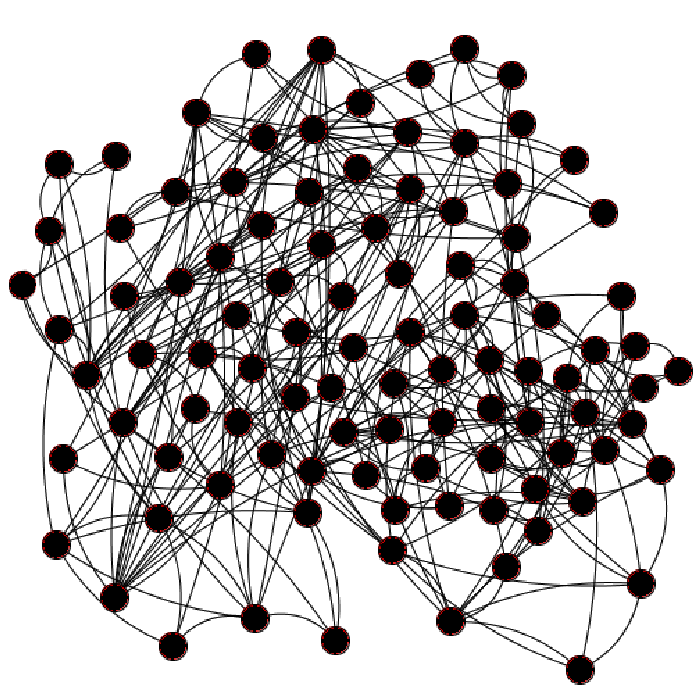
\includegraphics[width=0.8\textwidth]{newscastgraph}}
\caption{A snapshot of a newscast population structure for $c=4$ and $n=100$ (direction of the edges has been removed). It is straightforward to see that the node degree in newscast is smaller than in the panmictic case that would be represented by a complete graph with $\frac{n(n-1)}{2}$ edges.}
\label{fig:newscastsnapshot}
\end{figure*}
%%%%%%%%%%%%%%%%% 


\clearpage
%%%%%%%%%%%%%%%%%%%%%%%%%%%%%%%%%%%%%%%%%%%%%%%%%%%%%%%%%%%%%
\section{Practical issues}
\label{sec:practicalissues}
%%%%%%%%%%%%%%%%%%%%%%%%%%%%%%%%%%%%%%%%%%%%%%%%%%%%%%%%%%%%%

As previously explained, this thesis focuses on studying the viability of the \evag model from an algorithmic point of view. Nevertheless, this Section tries to provide some keys for the interpretation of results from a real-world application perspective in which the dominant time factor for an EA uses to be the fitness evaluation. Therefore, the following sections analyse the limitations on local and parallel performances imposed by the fitness evaluation cost and conditioned by the underlying computing platform.


%%%%%%%%%%%%%%%%%%%%%%%%%%%%%%%%
\subsection{Local performance}
\label{sec:localperformance}
%%%%%%%%%%%%%%%%%%%%%%%%%%%%%%%%

Locally to a computer, every \evag can be scheduled within a thread and dispatched by the operative system. The multi-threading nature of the model implies an impact on the local throughput, expressed as:

\begin{equation}
Throughput_{EA}=\frac{Computational \quad Effort}{Time}
\label{eq:throughput}
\end{equation}

\noindent where Computational Effort is usually understood in EC as the number of fitness evaluations.

Either the context exchange of the threads or the mutual exclusion mechanisms have a computational cost which is avoid in sequential approaches.

Nevertheless, Symmetric Multiprocessing (SMP) architectures are becoming nowadays very popular in desktop machines where sequential approaches are unable to take advantage of more than a single processor.
This way, the local performance of the \evag model can be assessed by measuring the speedup in the throughput with respect to a sequential GA (sGA):


\begin{equation}
\label{eq:speedup}
Speedup = \frac{Throughput_{EvAg}}{Throughput_{sGA}}
\end{equation}

To this end, the computational cost of the evaluation function (i.e. the independent variable in the throughput equation) is scaled from few milliseconds to one second.


\begin{figure*}[htbp]
\centering
\subfigure{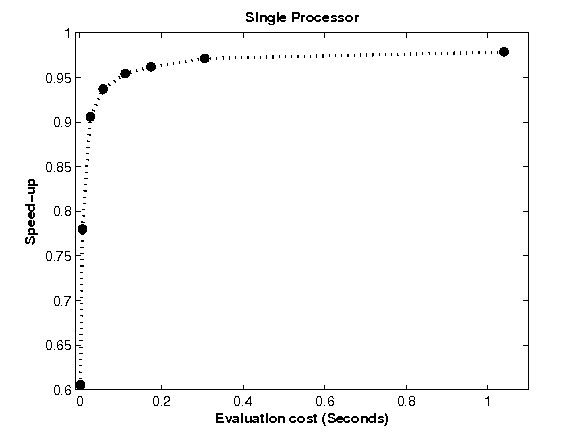
\includegraphics[width=0.7\textwidth]{single_sca}}\\
\subfigure{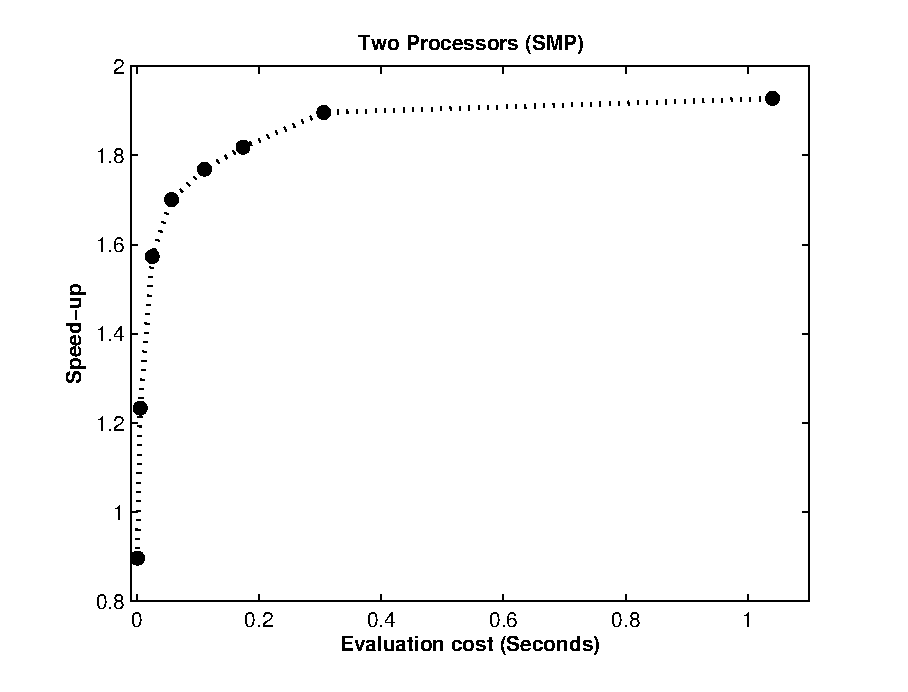
\includegraphics[width=0.7\textwidth]{smp_sca}}
\caption{The figure depicts how the \evag throughput speeds up with respect to the sGA one when the evaluation function cost scales for a population size of 400 individuals.
The test-bed is a single processor ({\em upper figure}) and a dual-core processor ({\em bottom figure}).}
\label{fig:sca}
\end{figure*}

Figure \ref{fig:sca} shows that the throughput speeds up asymptotically, having a limit on the number of processors. Therefore, the performance in single processor machines tends to be equivalent to sequential approaches as the evaluation cost increases while is clearly outperformed in SMP machines. An additional advantage of the \evag model is that the load balance at this level is transparent for the programmer since it is carried out by the operative system.

\clearpage
%%%%%%%%%%%%%%%%%%%%%%%%%%%%%%%%
\subsection{Parallel performance}
\label{sec:parallelperformance}
%%%%%%%%%%%%%%%%%%%%%%%%%%%%%%%%

In parallel infrastructures, the speedup is a commonly used metric to measure the parallel performance of a distributed algorithm over the sequential one. Gagn\'e et al. define in \cite{gagne:msperformance} the speedup of a distributed EA assuming that the fitness evaluation is the main consuming task:

\begin{equation}
Speedup = \frac{NT_f}{T_p}
\end{equation}

\noindent where $N$ is the population size, $T_f$ is the time needed to evaluate the fitness of a single individual and $T_p$ is the time needed to evaluate all the individuals using $P$ processors. 

In the case of a P2P system, every individual is placed in a single processor and therefore $P=N$ and $T_p= T_N$. Then:

\begin{equation}
T_{N} = \underbrace{T_f}_{computation} + \underbrace{\frac{N}{m}T_{comm}}_{communication} + \underbrace{T_{lat}}_{latency}
\end{equation}

\noindent where $T_{comm}$ is the communication time required by every \evag at each evolutionary cycle and $m$ is the number of hub/gateways of the physical network from which all the network traffic is dispatched. Being $T_{ind}$ the time to transmit a single individual, $T_{comm} = 2T_{ind}$ in the case of using a selection operator such as binary tournament. Finally, the latency time, $T_{lat}$, will depend on the infrastructure of the physical network. This way, having a single queue gateway $M/M/1$ (as depicted in Figure \ref{fig:singlequeue}), the latency time can be explained as the mean response time of the gateway \cite{jain:performanceanalysis}:

\begin{equation}
T_{lat_{M/M/1}}=\frac{\underbrace{\frac{1}{\mu}}_{throughput}}{1-\underbrace{\frac{\lambda}{\mu}}_{utilisation}}
\end{equation}

\noindent where $\lambda$ represents the incoming traffic rate and $\mu$ the throughput rate. This way, the traffic intensity (or utilisation of the gateway) can be expressed as $\rho=\frac{\lambda}{\mu}$ and the latency time  extended to $m$ gateways following a $M/M/m$ scheme:

\begin{equation}
T_{lat_{M/M/m}}=\frac{1}{\mu}(1+\frac{\rho}{m(1-\rho)})
\end{equation}


\begin{figure*}[htbp]
\centerline{
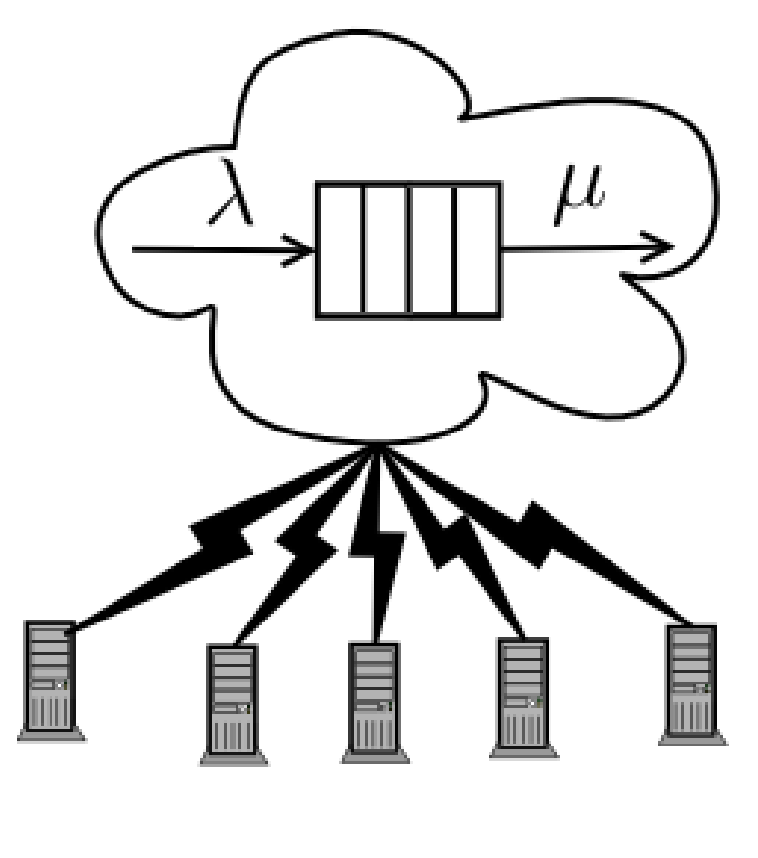
\includegraphics[width=0.4\textwidth]{queuemm1}
}
\caption{Scheme of a M/M/1 queueing system. $\lambda$ stands for the incoming traffic rate and $\mu$ for the throughput rate.}
\label{fig:singlequeue}
\end{figure*}


Under such a framework, the following experiment aims to provide a guideline on how the fitness evaluation cost and the underlying computing platform may influence the parallel performance of the \evag approach. 

According to Thierens in \cite{thierens:scalability}, the population size of an EA ($N$) roughly scales with an order $O(l^\alpha)$, where $l$ is the chromosome length in bits and $\alpha$ is a constant that depends on the algorithm and the problem complexity. Therefore, we can analyse the parallel performance of our P2P EA model under the following assumptions by scaling $l \in [1\dots100]$:

\begin{itemize} 
\item Since $N$ scales with an order $~O(l^\alpha)$, we have set $N=l^\alpha$. Taking into account the empirical results on the Thierens paper, a problem of intermediate difficulty can scale with $\alpha=2$. 

\item We assume that $T_{ind}=l$, meaning that the time to transmit an individual through the network scales linearly with respect to the chromosome length.

\item Given that $\lambda$ represents the incoming traffic rate in a gateway, it can be explained by $\lambda=\frac{N}{m}2T_{ind}$ if we assume a perfect load balancing of all communications through the $m$ gateways.

\item $\mu$ has been adjusted to $20000$ in such a way that the single gateway queueing $M/M/1$ would suffer overflow beyond $l=100$.

\item To analyse the influence of the fitness evaluation cost and the network infrastructure on the speedup, we have considered six possible scenarios for both variables:

\begin{itemize}
\item The fitness evaluation cost is obviously a problem-dependent variable. In real-world problems, the complexity orders tend to be high. Therefore, by simply assuming polynomial orders of complexity $O(l^\zeta)$, the fitness evaluation can be expressed as $T_f=l^\zeta$. This experiment consider $\zeta=[\frac{3}{2},2,3]$  which are rather optimistic values considering real-world problems.

\item In order to assess the influence of the physical network on the parallel performance, we consider two possible infrastructures, the first using a single queue gateway $m=1$ (as it could be the case in a LAN) and the second one using a eight queueing system $m=8$.
\end{itemize}

\end{itemize}


\begin{figure*}[htbp]
\centering
\subfigure{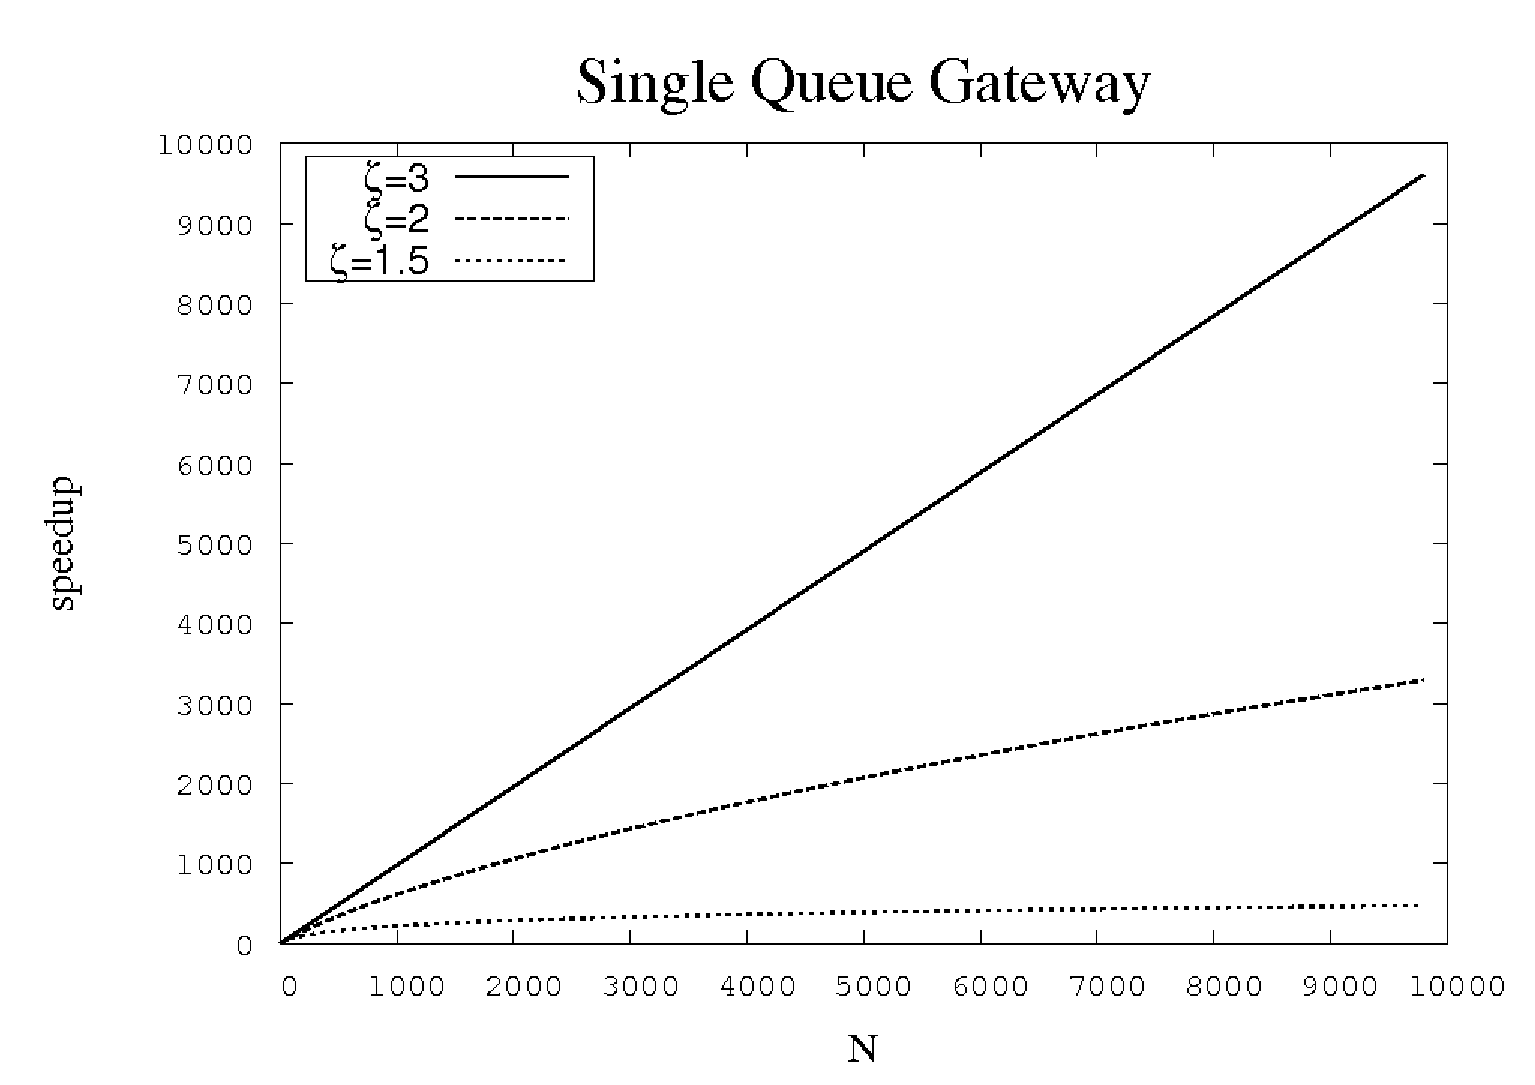
\includegraphics[width=0.7\textwidth]{mm1}}\\
\subfigure{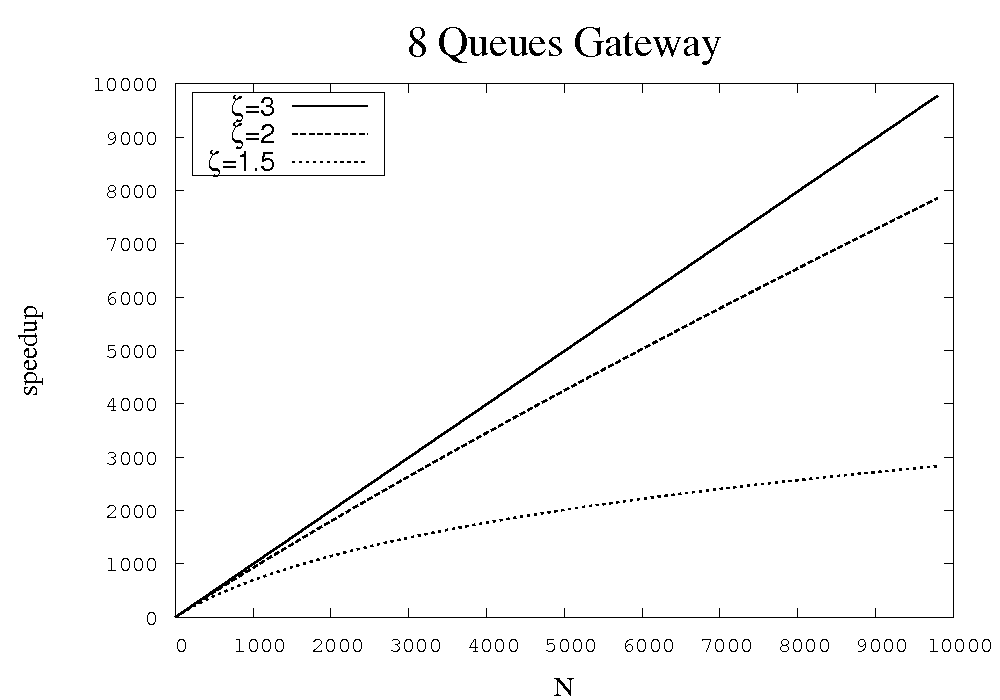
\includegraphics[width=0.7\textwidth]{mm8}}
\caption{ Speedup curves for $\zeta=[\frac{3}{2},2,3]$ as a function of the population size (or alternatively the number of processors since $N=P$). Results are obtained for a single queue gateway architecture ({\em up}) and a 8 queues gateway system ({\em down}).}
\label{fig:parallelperformance}
\end{figure*}

Figure \ref{fig:parallelperformance} shows the maximum speedup that the P2P approach can reach on every of the six scenarios under study. Beyond the numerical fit of the assumptions, results provide a qualitative estimation on how the fitness evaluation cost and the underlying computing platform influence the performance.

On the one hand, the scalability of the fitness evaluation cost is key to hold linear speedups. In addition, not all the problem instances but those requiring larger genomes can apply for massive parallelisation. In this sense, the scalability of the population size impose a limitation on the number of processors to be used since $P=N$ at a higher bound. On the other hand, the underlying architecture plays an important role on the communication time and therefore on the overall performance. It can be seen how the problems  scaling with sublinear speedups (e.g. for $\zeta=2$) perform much better for infrastructures with a higher capacity.

\clearpage
\section{Summary}
%%%%%%%%%%%%%%%%%%%%%%%%%%%%%%%%%%%%%%%%%%%%%%%%%%%%%%%%%%%%%%


The Evolvable Agent model is a fine-grained spatially-structured EA composed of a population of Agents. Every \evag acts at two levels; evolving a single individual with the mate selection locally restricted within a neighbourhood and dynamically structuring such a neighbourhood by means of the protocol newscast.  This makes the approach suitable for a P2P execution in which every \evag can be potentially placed in a different peer. In such a loosely-coupled scenario, the execution of the model is decentralised and lacks of a central clock which implies the asynchronous evolution of the individuals.

Inherent to the model is that such an asynchronous execution allows to take a seamless advantage of the several processors in SMP computers, outperforming, this way, the throughput of a sequential EA for demanding fitness evaluation functions. Additionally, the parallel performance of the model has been shown to scale up to thousands of computers with a linear speedup. Nevertheless, it has to be taken into account that such a case would require of a highly expensive fitness evaluation, a large number of individuals and a parallel infrastructure able to support all the network traffic.

Therefore, to this point, massive scalability of the \evag model remain in an idealised scenario that do not account for the algorithmic issues of the approach itself, such as the asynchrony, nodes failures or dynamic changes on the population structure. This way, the following chapter will tackle the {\em algorithmic performance} of the model from the perspective of the experimental analysis.
%, showing whether the algorithm is able to converge to convenient solutions despite the asynchrony, nodes failures or dynamic changes on the population structure. 
%This way, the following chapter proposes a methodology for the analysis of the algorithm in a simulated P2P environment so that the viability of the P2P EA can be drawn from the algorithmic performance of the approach.


%%%%%%%%%%%%%% Bibliografia %%%%%%%%%%%%%%%

%\bibliographystyle{alpha}  % Eliminarlo al compilar el documento maestro, ponerlo para compilarlo separado
%\bibliography{pea,p2pcomputing,model}% Eliminarlo al compilar el documento maestro, ponerlo para compilarlo separado

%\end{document}             % Eliminarlo al compilar el documento maestro, ponerlo para compilarlo separado%

